\section{XAI in Autonomous Vehicles}\label{sec:Alignment}

\subsection{Existing Research}

In one study, research subjects participated in a driving simulator in which the vehicle had a semi-autonomous feature that would initiate hard braking events in the case of an unforeseen obstacle in the path of the vehicle \cite{Koo2015}.  Researchers programmed the simulator to provide different types of verbal explanations for the hard brake events.  Survey responses from the research subjects showed that drivers had not only more positive emotional responses when more descriptive explanations were provided by the semi-autonomous system, but there was also measurably safer driving habits observed by the drivers when they received rich explanations that described not only how the vehicle was behaving but also why it was choosing those behaviors.

It is not uncommon for researchers to generate saliency maps of feature importance when doing computer vision tasks with deep neural networks.  These feature saliency maps can overlay neatly over the original image to help developers of these decision systems to identify if the responses from the neural network are behaving as expected.  Bojarski et al. developed a method of generating saliency maps called VisualBackProp \cite{DBLP:journals/corr/BojarskiCCFJMZ16} and apply it to an end-to-end autonomous driving system called PilotNet.  PilotNet can decide steering wheel angles given input images, bypassing the need for an intermediate perception phase that identifies segmented objects in images before making decisions.  VisualBackProp confirms that PilotNet is making decisions based on human-understandable features in the images, such as the boundaries of the road, lane markers, and the boundaries of other vehicles on the road (see figure \ref{fig:bojarski2017}) \cite{Bojarski2017ExplainingHA}.

\begin{figure}
    \centering
    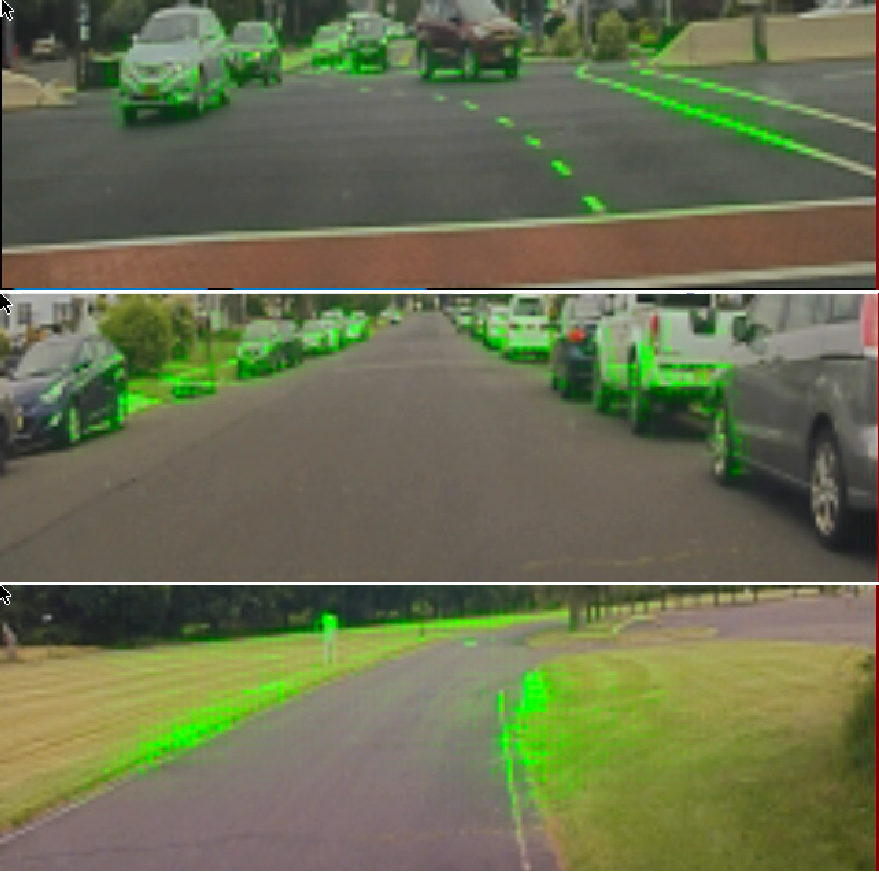
\includegraphics[width=3.4in]{media/bojarski2017.png}
    \caption{Bojarski et al. generate saliency maps of input features in their end-to-end autonomous driving system \cite{Bojarski2017ExplainingHA}}
    \label{fig:bojarski2017}
\end{figure}

Using visual explanations to explain the decisions of a trained model has multiple drawbacks which can be ameliorated with the emerging method of verbalization in XAI.  While saliency maps may give insight into how a model is responding to a single input, both humans and autonomous systems make decisions based on information over time.  Also, the interpretation of a visual explanation is subjective to the human audience; different observers may draw different or no insights from a single visual explanation.  Kim et al. train a LSTM neural net on a dataset of images over time accompanied by human-labeled explanations of the current driving behavior \cite{kim2018textual}.  The output layer of this trained model labels images over time with descriptive natural language of the driving behavior.  Provided as input into this verbalization model are "attention" maps of regions in the images that are identified as important features.  These regions of high and weak attention are generated from a CNN that is used to decide acceleration and course change behavior given input images.  The objective of Kim et al. of explaining a limited set of automated behavior in an autonomous vehicle via visual explanations is similar to the work of Bojarski et al \cite{Bojarski2017ExplainingHA}, but the concept is taken further by generating natural language responses to the feature relevances over time.

\begin{itemize}
    \item There are a couple papers about the multimodal sensors in AV, the perception/decision architecture, and a survey of decision 
    \item There are quite a few papers about establishing trust with automated systems, AI, and HCI.  Is there a gap in establishing trust that has not been addressed in previous research?
    \item Might have to put the legal/auditory use case on the back burner...way out of scope for my expertise at this time.
\end{itemize}

\subsection{Future Research in Use Case \ref{subsec:UseCase1}}

One of the most explicit use cases for applying XAI methods to the domain of autonomous vehicles is in the support of researchers and engineers to develop more accurate and robust machine learning models, especially in the perception and decision systems of the autonomous vehicle.  In the use case defined in \ref{subsec:UseCase1}, we identified examples of data scientists using explanations of non-intuitive, black-box ML models to improve how the models were trained and thus improve the performance of the models.  While some researchers have applied XAI to CNNs that were used in an end-to-end system to decide steering angles \cite{Bojarski2017ExplainingHA}, there was no published research found at the time of this writing on applying XAI towards the improvement of CNNs being applied in the perception system of autonomous vehicles for tasks such as object detection and object segmentation.  In the decision systems of autonomous vehicles, deep reinforcement learning is an emerging field for the training of autonomous vehicles \cite{Sallab2017DeepRL}, and the resulting deep q-networks (DQNs) have not been explored for explaining their decisions onto a human-interpretable domain.  Besides using explanations to discover opportunities to improve models, there is no published research on the application of data provenance as a tool to assist with the ML workflow of developers of autonomous vehicles through collaboration and reproduction of experiments.

\subsection{Future Research in Use Case \ref{subsec:UseCase2}}

Trust in autonomous vehicles has been identified as having a positive, causal relationship with people's intention to use autonomous vehicle technology \cite{Choi2015InvestigatingTI}.  The influence of trust in the intention of using AV technology was broken down into various constructs (see figure /ref{fig:choi2015}), and XAI may be applicable to two of those constructs in particular:  system transparency and situation management.  System transparency may be the least influential construct of trust, but it would likely be the most directly applicable area for XAI.  XAI methods such as rule extraction for the decision system and verbalization techniques for the perception system may be able to map the predictions and decisions of the AV system onto the human interpretable domain of natural language.  Two aspects of situation management include the system's ability to generate alternative decisions and the user's ability to control the autonomous vehicle.  Rule-based and fuzzy decision systems can inherently provide a ranked ordering of other alternative decisions that were considered, and simple labeling of which decisions were made by the autonomous systems and which decisions were provided by the user can provide users with explanations on the system's situation management.  It may be valuable to observe the impact of the application of XAI methods on these constructs of trust in the user experience of users of AV systems.

\begin{figure*}
    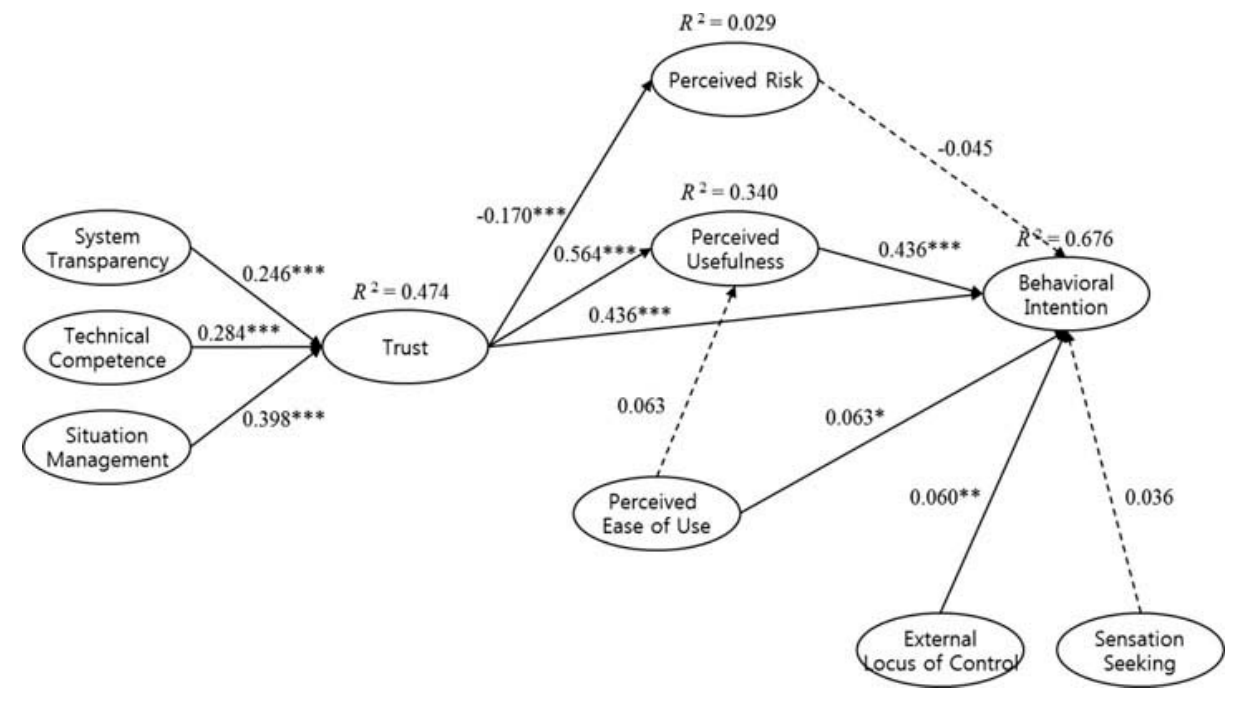
\includegraphics[width=\textwidth]{media/choi2015}
    \caption{Choi et al. break down the constructs of trust and influences on people's behavioral intention of using AV technology \cite{Choi2015InvestigatingTI}  \textit{Note:} *p < .05. **p < .01. ***p < .001.}
    \label{fig:choi2015}
\end{figure*}

\subsection{Future Research in Use Case \ref{subsec:UseCase3}}

The legal impetus of explaining the decisions made by autonomous vehicles is often not present in regional legislation or is at risk of being unenforceable due to lack of clarity or definition.  The US Department of Transportation's National Highway Traffic Safety Administration has released guidelines on the development and adoption of autonomous vehicles which defer legislation to state or municipal bodies \cite{USDOT2018}, and currently, 14 states and no US territories have put legislation into law regarding autonomous vehicles \cite{ncsl}.  California has a dedicated Department of Autonomous Vehicles which has regulation around the reporting of collisions and disengagements of autonomous vehicle systems in the state, but the requirements for describing the cause of disengagements lacks any requirements on explaining the autonomous decision system \cite{CalDMV}.  In the EU, the General Data Protection Regulation (GDPR) contains recitals that grant consumers the right to request what data of theirs companies are collecting, how companies are using it, and how decisions with their data are made.  While some aspects of the GDPR are conceptually more straight-forward, such as consumers requesting the data of theirs that a company has collected, there is a lack of definition and clarity around the idea of explaining decisions that companies make with consumers' data, and it is unclear if the GDPR's so-called "right to explanation" is enforceable \cite{Mittelstadt2017}.  The future task of effectively legislating and enforcing fair, accountable, and transparent machine learning algorithms is uncertain and daunting.

First steps in approaching the modernization of the relationship between legislation and AI/ML in autonomous vehicles may include designing autonomous vehicle systems to be able to store and extract data and metadata for all relevant stakeholders, the identification of regulatory and legislative gaps on autonomous vehicles, and establishing effective language to make laws and regulations enforceable for accountable and transparent decision systems in autonomous vehicles.  Stakeholders of decisions from autonomous systems can be expert users or lay users, and lay users can be anyone from the consumer of the autonomous system to individuals in the public who are acting as input to the autonomous vehicle's perception systems \cite{Ras2018ExplanationMI}.  The challenge of how to design systems to make decision and explanation data for such a wide variety of stakeholders may be an emerging area of research in the explainability of autonomous vehicle systems.  While some geographic regions explicitly lack any legislation or regulation on autonomous vehicles, even the regions that do have laws in place may find them difficult or ineffective to enforce \cite{Mittelstadt2017}.  Wachter et al. establish eight recommendations for strengthening the "right to explanation" in the GDPR, including clarification on if the consumers' "right to access" from Article 15 of the GDPR includes the explanation or just the existence of a decision, what metadata on the decision process constitutes an explanation (feature importance, decision tree model, etc.), when a decision is based solely on an automated process.  The future of the legal aspect of explainable autonomous systems will be a combination of designing systems for data extraction and the refinement of laws and regulations.
